\documentclass{article}

\usepackage[english]{babel}
\usepackage{graphicx}
\usepackage{framed}
\usepackage[normalem]{ulem}
\usepackage{indentfirst}
\usepackage{amsmath,amsthm,amssymb,amsfonts}
\usepackage{mathtools} % Wraparound amsmath. For fancy math typesetting
\usepackage[nointegrals]{wasysym} % nointegrals prevents wasysym from overwriting integral symbols from LaTeX and amsmath
\usepackage{bbm} % For extended bold and blackboard bold characters
\usepackage[italicdiff]{physics} % italicdiff causes derivatives to be rendered with italic d's instead of upright d's
\usepackage[T1]{fontenc}
\usepackage{xparse}
\usepackage{xstring}
\usepackage{xspace}
% \usepackage{pifont} % For unusual symbols
% \usepackage{mathdots} % For unusual combinations of dots
\usepackage{stmaryrd} % For \llbracket and \rrbracket (ring of formal power series)
\usepackage{nicematrix}
\usepackage{fontawesome5} % For fancy graphic symbols
\usepackage{wrapfig}
\usepackage{lmodern,mathrsfs}
\usepackage[inline,shortlabels]{enumitem}
\setlist{topsep=2pt,itemsep=2pt,parsep=0pt,partopsep=0pt}
\usepackage[table,dvipsnames]{xcolor}
\usepackage[utf8]{inputenc}
\usepackage{csquotes} % Must be loaded AFTER inputenc
\usepackage{imakeidx}
\makeindex[intoc,title={Index}]
\usepackage[a4paper,top=0.7in,bottom=0.7in,left=0.5in,right=0.5in]{geometry}
\usepackage[most]{tcolorbox}
\usepackage{tikz,tikz-3dplot,tikz-cd,tkz-tab,tkz-euclide,pgf,pgfplots}
\usetikzlibrary{shapes}
\pgfplotsset{compat=newest}
\usepackage{subfiles}
\graphicspath{{images/}{../images/}} % To allow rendering of images from the main file as well as subfiles
% \usepackage{comment} % For commenting large blocks of text and math efficiently
% \usepackage{fancyvrb} % For custom verbatim environments
\usepackage{multicol}
\usepackage[bottom,multiple]{footmisc} % Ensures footnotes are at the bottom of the page, and separates footnotes by a comma if they are adjacent
\usepackage[backend=bibtex,style=numeric]{biblatex}
\renewcommand*{\finalnamedelim}{\addcomma\addspace} % Forces authors' names to be separated by comma, instead of "and"
% \addbibresource{bibliography}
\usepackage{minted} % Allows input of raw code, such as Python code
\usepackage{xurl} % Allows more control over urls, such as line breaks within a url
\usepackage[colorlinks,linkcolor=.,citecolor=blue,urlcolor=violet]{hyperref}
\usepackage[nameinlink]{cleveref} % nameinlink ensures that the entire element is clickable in the pdf, not just the number

% Local packages to be loaded %
\usepackage{commands}
\usepackage[inplace]{exercise_format}
\usepackage{labeled_boxes}
\usepackage{matrices}
\usepackage{python_boxes}
\usepackage{theorems}
\usepackage{timestamps}
\usepackage{number_rings}

% \makeatletter

% % Internal storage: \thmnamestore@<label> holds the name
% \def\@storetheoremname#1#2{%
%   % #1 = label, #2 = name
%   \expandafter\gdef\csname thmnamestore@#1\endcsname{#2}%
% }

% % Hook into \label to capture the current theorem name at label-time
% \let\orig@label\label
% \renewcommand{\label}[1]{%
%   \orig@label{#1}%
%   \ifdefined\@currenttheoremname
%     \ifx\@currenttheoremname\@empty\else
%       \@storetheoremname{#1}{\@currenttheoremname}%
%     \fi
%   \fi
% }

% % Hook into amsthm to set \@currenttheoremname, clear it after the env
% \let\orig@thm\@thm
% \def\@thm#1#2#3{%
%   \def\@currenttheoremname{#3}%
%   \orig@thm{#1}{#2}{#3}%
% }

% % Clear the name after the theorem body ends
% \let\orig@endtheorem\@endtheorem
% \def\@endtheorem{%
%   \orig@endtheorem
%   \let\@currenttheoremname\@undefined
% }

% % \Nref{label}: link using stored name, error if absent
% \NewDocumentCommand{\Nref}{m}{%
%   \ifcsname thmnamestore@#1\endcsname
%     \hyperref[#1]{\csname thmnamestore@#1\endcsname}%
%   \else
%     \PackageError{Nref}{%
%       \string\Nref\space used on label '#1', but this theorem has no name%
%     }{%
%       Add an optional name argument: \string\begin{theorem}[Name]\string\label{#1}%
%     }%
%   \fi
% }

% \makeatother

\newcommand{\remind}[1]{\textcolor{red}{\textbf{#1}}} % To remind me of unfinished work to fix later
\newcommand{\hide}[1]{} % To hide large blocks of code without using % symbols

% Same as \href, but the text appears in typewriter font and in a custom color
\newcommand{\Href}[3][red!50!black]{\href{#2}{\textcolor{#1}{\texttt{#3}}}}

\usepackage{fancyhdr}
% To set the header and footer on each page
\fancyhead[L]{\sffamily\nouppercase{\leftmark}}
% \fancyhead[R]{\sffamily\nouppercase{\rightmark}}
% \fancyhead[R]{\sffamily\itshape Version of \DTMToday, \DTMcurrenttime \ (\DTMcurrentzone)}
\fancyhead[R]{\sffamily\faCalendar* \ \DTMToday \hspace{\fsize} \faClock \ \DTMcurrenttime \ (\DTMcurrentzone)}
\fancyfoot[C]{\sffamily\thepage}
\renewcommand{\headrulewidth}{0.5pt}
\renewcommand{\footrulewidth}{0.5pt}
\setlength{\headheight}{15pt}
\pagestyle{fancy}

% To set the footer on the first page of each chapter
\fancypagestyle{plain}{
\fancyhf{}
\renewcommand{\headrulewidth}{0pt}
\renewcommand{\footrulewidth}{0pt}
\fancyfoot[C]{\sffamily\thepage}}

\setcounter{section}{-1}

\makeatletter
% Redefining the title block
\renewcommand{\maketitle}{%
    \thispagestyle{empty}
    \begin{center}
        \null\vspace{2mm}
        {\fontsize{24}{28}\sffamily\bfseries\selectfont\@title}\\
        \vspace{6mm}
        {\fontsize{20}{24}\sffamily\selectfont\@author}
    \end{center}
}
\makeatother

\title{math-blurbs}
\author{self-adjoint}
\date{\DTMToday}

\begin{document}

\maketitle

\VersionTimestamp

This project is hosted on GitHub: \url{https://github.com/self-adjoint/math-blurbs}

\section{Introduction}

\subsection{The QED Symbol}

\href{https://mathworld.wolfram.com/QED.html}{QED} stands for \emph{quod erat demonstrandum} (Latin for ``that which was to be demonstrated''), and is used to signify the end of a mathematical proof. Most mathematicians use either a white square $\square$ or a black square $\blacksquare$ for this. \href{https://news.uchicago.edu/story/paul-j-sally-jr-influential-mathematician-and-educator-1933-2013}{Paul J., Sally, Jr.} (1933 -- 2013) famously used a sketch of himself in an eyepatch\footnote{He was legally blind in his left eye, and nicknamed ``The Math Pirate'' and ``Professor Pirate'' by his students.} as the QED symbol in his books.

\begin{theorem}
    For any group of people, there are at least two people with the same number of friends.
\end{theorem}
\begin{proof}
    Suppose there are $n$ people in the group. Each person can have any number of friends from $0$ to $n-1$ (so there are $n$ possible values). However, there cannot be both a person with $0$ friends (friends with no one) and a person with $n-1$ friends (friends with everyone). Thus, there must be at least two people with the same number of friends.
\end{proof}

The QED symbol I have chosen to use is the \href{https://emojipedia.org/smiling-face-with-sunglasses}{Smiling Face with Sunglasses} emoji\footnote{Not to be confused with an \href{https://www.britannica.com/story/whats-the-difference-between-emoji-and-emoticons}{emoticon}, which refers to things like :) and :( and were mainly used before emojis were introduced into \href{https://emojipedia.org/unicode-6.0}{Unicode 6.0}.}. This version has been used by \href{https://www.whatsapp.com/}{WhatsApp} since 2017.

\begin{theorem}[Cool thing]\label{lookatme}
    This is a theorem
\end{theorem}

\Cref{lookatme}

% \Nref{lookatme}
\newpage
\section{Limit inferior and limit superior}

\begin{definition}
    Suppose $(a_n)_{n=1}^\infty$ is a sequence in $\R$. The \textbf{limit inferior} and \textbf{limit superior} of $(a_n)_{n=1}^\infty$ respectively are given by:
    \begin{align*}
        \liminfn a_n = \sup_{n\in\N} \inf_{k\ge n} a_k && \limsupn a_n = \inf_{n\in\N} \sup_{k\ge n} a_k
    \end{align*}
    Note that $\liminfn a_n$ and $\limsupn a_n$ are allowed to be $\pm\infty$.
\end{definition}

\begin{exercise}
    Suppose $(a_n)_{n=1}^\infty$ is a sequence in $\R$ and $x\in\R$. Prove that:
    \begin{enumerate}
        \item $x<\liminfn a_n$ if and only if $x<a_n$ for all but finitely many $n\in\N$.
        \item $x<\limsupn a_n$ if and only if $x<a_n$ for infinitely many $n\in\N$.
    \end{enumerate}
    Do these statements hold if we replace the strict inequalities with non-strict inequalities? Prove or give a counterexample for each one.
\end{exercise}

\begin{exercise}\label{liminf_limsup_inequalities}
    Suppose $(a_n)_{n=1}^\infty$ and $(b_n)_{n=1}^\infty$ are sequences in $\R$. Prove that:
    \begin{equation*}
        \liminfn a_n + \liminfn b_n
        \le \liminfn (a_n+b_n)
        \le \liminfn a_n + \limsupn b_n
        \le \limsupn (a_n+b_n)
        \le \limsupn a_n + \limsupn b_n
    \end{equation*}
    For each inequality, give an example of sequences $(a_n)_{n=1}^\infty$ and $(b_n)_{n=1}^\infty$ where it is strict. Can you find a single example of $(a_n)_{n=1}^\infty$ and $(b_n)_{n=1}^\infty$ where \emph{all four} inequalities are strict?
\end{exercise}

\begin{definition}
    Suppose $(A_n)_{n=1}^\infty$ is a sequence of subsets of $\R$. The \textbf{limit inferior} and \textbf{limit superior} of $(A_n)_{n=1}^\infty$ respectively are given by:
    \begin{align*}
        \liminfn A_n = \cuppn \capp_{k\ge n} A_k && \limsupn A_n = \cappn \cupp_{k\ge n} A_k
    \end{align*}
\end{definition}

\begin{exercise}
    Suppose $(A_n)_{n=1}^\infty$ is a sequence of subsets of $\R$ and $x\in\R$. Prove that:
    \begin{enumerate}
        \item $x\in\liminfn A_n$ if and only if $x\in A_n$ for all but finitely many $n\in\N$.
        \item $x\in\limsupn A_n$ if and only if $x\in A_n$ for infinitely many $n\in\N$.
    \end{enumerate}
\end{exercise}

\begin{exercise}
    State and prove an analog of \Cref{liminf_limsup_inequalities} for sequences of subsets of $\R$.
\end{exercise}

\begin{definition}
    A function $f:\R\to\R$ is \textbf{additive} if $f(x+y)=f(x)+f(y)$ for all $x,y\in\R$.
\end{definition}
\begin{remarks}\leavevmode
    \begin{enumerate}
        \item The equation $f(x+y)=f(x)+f(y)$ is known as the \textit{Cauchy functional equation}.
        \item It follows by replacing $x$ with $x-y$ that $f(x-y)=f(x)-f(y)$ for all $x,y\in\R$. It then follows by substituting $x=y$ that $f(0)=0$.
    \end{enumerate}
\end{remarks}

\begin{lemma}\label{additiverational}
    Suppose $f:\R\to\R$ is additive. Then $f(cx)=cf(x)$ for all $c\in\Q$ and all $x\in\R$.
\end{lemma}
\begin{proof}
    Suppose $x\in\R$. We first show that $f(nx)=nf(x)$ for all $n\in\Z$. Clearly this holds for $n=1$ as both sides reduce to $f(x)$. Suppose the equation holds for some $n\in\Z$. Then we have:
    \begin{align*}
        f((n+1)x)&=f(nx+x)=f(nx)+f(x)=nf(x)+f(x)=(n+1)f(x) \\
        f((n-1)x)&=f(nx-x)=f(nx)-f(x)=nf(x)-f(x)=(n-1)f(x)
    \end{align*}
    Thus the equation holds for $n+1$ and $n-1$, and so it holds for all $n\in\Z$.\\
    
    Now suppose $c\in\Q$. Then $c=\frac{p}{q}$ for some $p,q\in\Z$, $q\ne0$. By what we have just shown, we have $f(px)=pf(x)$ and $f(qy)=qf(y)$ for all $x,y\in\R$. Substituting $y=\frac{x}{q}$ yields $f(x)=qf\big(\frac{x}{q}\big)$, i.e. $f\big(\frac{x}{q}\big)=\frac{1}{q}f(x)$, and so $f\big(\frac{p}{q}x\big)=\frac{p}{q}f(x)$. Thus $f(cx)=cf(x)$ for all $c\in\Q$ and all $x\in\R$.
\end{proof}

\begin{proposition}\label{additivelmcont0}
    If $f:\R\to\R$ is additive and Lebesgue measurable, then $f$ is continuous at $0$.
\end{proposition}
\begin{proof}
    Suppose $U\sub\R$ is an open set containing $0$ and $V\sub U$ is an open set such that $\{x-y\mid x,y\in V\}\sub U$. Also suppose $(q_n)_{n=1}^\infty$ is an enumeration of $\Q$. Then we have $\cuppn(q_n+V)=\R$, and so $\cuppn f^{-1}(q_n+V)=\R$ as well. For each $n\in\N$, define $W_n=f^{-1}(q_n+V)$. Then we have $\cuppn W_n=\R$, so $\mu(W_n)>0$ for at least one $n\in\N$. By Sierpinski's theorem on sets of differences, the set $\{x-y\mid x,y\in W_n\}$ contains $(-\ep,\ep)$ for some $\ep>0$. Since $\{x-y\mid x,y\in W_n\}\sub f^{-1}(\{x-y\mid x,y\in V\})\sub f^{-1}(U)$, it follows that $f^{-1}(U)$ contains $(-\ep,\ep)$. Thus $f$ is continuous at $0$.
    % https://math.stackexchange.com/questions/359183/measurable-cauchy-function-is-continuous
\end{proof}

\begin{lemma}\label{additivec1p}
    If $f:\R\to\R$ is additive and continuous at one point, then it is continuous on $\R$.
\end{lemma}
\begin{proof}
    Suppose $f$ is continuous at some $a\in\R$. Then we have $\limx f(x)=f(a)$. For any $b\in\R$, we have:
    \begin{equation*}
        \lim_{x\to b} f(x)=\lim_{x\to a} f(x-a+b)=\lim_{x\to a} (f(x)-f(a)+f(b))=\lim_{x\to a} f(x)-f(a)+f(b)=f(b)
    \end{equation*}
    Thus $f$ is continuous at every $b\in\R$.
\end{proof}

\begin{proposition}\label{additivecont}
    Suppose $f:\R\to\R$ is additive and continuous. Then there is a constant $a\in\R$ such that $f(x)=ax$ for all $x\in\R$.
\end{proposition}
\begin{proof}
    Define $a=f(1)$. By \Cref{additiverational}, we have $f(cy)=cf(y)$ for all $c\in\Q$ and all $y\in\R$. Setting $y=1$ yields $f(c)=cf(1)=ac$. Suppose $x\in\R$ and $(q_n)$ is a sequence in $\Q$ that converges to $x$. Since $f$ is continuous, the sequence $(f(q_n))$ converges to $f(x)$. This yields $f(x)=\limn f(q_n)=\lim aq_n=a\limn q_n=ax$. Thus $f(x)=ax$ for all $x\in\R$.
\end{proof}

\begin{theorem}\label{additivelm}
    Suppose $f:\R\to\R$ is additive and Lebesgue measurable. Then there is a constant $a\in\R$ such that $f(x)=ax$ for all $x\in\R$.
\end{theorem}
\begin{proof}
    By \Cref{additivelmcont0}, $f$ is continuous at $0$, so by \Cref{additivec1p}, it is continuous on $\R$, and so by \Cref{additivecont}, we have $f(x)=ax$ for all $x\in\R$, where $a=f(1)$ is a constant.
\end{proof}

\begin{corollary}
    Suppose $f:\R\to\R$ is Lebesgue measurable and $f(x+y)=f(x)f(y)$ for all $x,y\in\R$. Then either $f\equiv0$ or there is a constant $a>0$ such that $f(x)=a^x$ for all $x\in\R$.
\end{corollary}
\begin{proof}
    Clearly $f\equiv0$ satisfies the above conditions. Note that if $f(x)=0$ for some $x\in\R$, then $f(x+y)=0f(y)=0$ for all $y\in\R$, and so $f\equiv0$. Suppose $f\not\equiv0$. Then $f(x)\ne0$ for all $x\in\R$. Moreover, we have $f(x)>0$ for all $x\in\R$, since $f(x)=f\left(\frac{x}{2}\right)^2$. Define $g:\R\to\R$ by $g(x)=\ln(f(x))$. This is well-defined as $f(x)>0$ for all $x\in\R$. We also have $g(x+y)=\ln(f(x+y))=\ln(f(x)f(y))=\ln(f(x))+\ln(f(y))=g(x)+g(y)$. Thus $g$ is additive. It is also Lebesgue measurable as $g=\ln(f)$ and $\ln$ is continuous. By \Cref{additivelm}, we have $g(x)=bx$ for all $x\in\R$, where $b=g(1)$ is a constant. Thus $f(x)=e^{bx}=a^x$ for all $x\in\R$, where $a=e^b$.
\end{proof}

Since $\R$ is a vector space over $\Q$, it has a basis. In other words, there is a set $\Bs\sub\R$ such that every $x\in\R$ can be expressed uniquely as $x=q_1x_1+q_2x_2+\cdots+q_nx_n$, where $x_1,x_2,...,x_n\in\Bs$ and $q_1,q_2,...,q_n\in\Q$. We now assign arbitrary values to $f(b)$ for every $b\in\Bs$. Since $\Bs$ is linearly independent over $\Q$, the value of $f(b)$ for any given $b\in\Bs$ is not affected by the values of $f$ at other points in $\Bs$, i.e. whatever values $f$ takes at points in $\Bs$, they will not contradict the equation $f(x+y)=f(x)+f(y)$. Also, since $\Bs$ spans $\R$, the values of $f$ at points in $\Bs$ uniquely determine its values at every point in $\R$.

\begin{definition}
    Suppose $I\sub\R$ is an interval. A function $f:I\to\R$ is \textbf{midpoint convex} (or \textit{Jensen convex} or \textit{midconvex}) on $I$ if $f\left(\frac{x+y}{2}\right)\le\frac{f(x)+f(y)}{2}$ for all $x,y\in I$.
\end{definition}
\begin{remark}
    It follows directly (by setting $\lam=\frac{1}{2}$ in the definition of a convex function) that every convex function is midpoint convex.
\end{remark}



\begin{theorem}
    If $f:I\to\R$ is midpoint convex and continuous, then $f$ is convex.
\end{theorem}
\begin{proof}
    Since $f$ is midpoint convex, for any $x,y\in I$, we have $f\left(\frac{x+y}{2}\right)\le\frac{f(x)+f(y)}{2}$. Since $I$ is an interval, we also have $\frac{x+y}{2}\in I$. This implies:
    \begin{align*}
        f\left(\frac{3}{4}x+\frac{1}{4}y\right)
        &=f\left(\frac{1}{2}\left(\frac{x+y}{2}+y\right)\right)
        \le\frac{1}{2}\left(f\left(\frac{x+y}{2}+f(y)\right)\right)
        \le\frac{1}{2}\left(\frac{f(x)+f(y)}{2}+f(y)\right)
        =\frac{3}{4}f(x)+\frac{1}{4}f(y)
        \\
        f\left(\frac{1}{4}x+\frac{3}{4}y\right)
        &=f\left(\frac{1}{2}\left(x+\frac{x+y}{2}\right)\right)
        \le\frac{1}{2}\left(f(x)+f\left(\frac{x+y}{2}\right)\right)
        \le\frac{1}{2}\left(f(x)+\frac{f(x)+f(y)}{2}\right)
        =\frac{1}{3}f(x)+\frac{1}{4}f(y)
    \end{align*}
    Repeating this process, we have for all $n\in\N$ and all $m\in\{0,1,...,2^n\}$:
    \begin{equation*}
        f\left(\frac{m}{2^n}x+\left(1-\frac{m}{2^n}\right)y\right)
        \le\frac{m}{2^n}f(x)+\left(1-\frac{m}{2^n}\right)f(y)
    \end{equation*}
    Now suppose $x,y\in I$ and $\lam\in[0,1]$. Then there is a sequence $(q_n)$ of rational numbers in $[0,1]$ with denominators $2^n$ that converges to $\lam$, e.g. $q_n=\frac{\lfloor 2^n\lam\rfloor}{2^n}$. For each $n\in\N$, we have $f(q_nx+(1-q_n)y)\le q_nf(x)+(1-q_n)f(y)$. As $n\to\infty$, the right side tends to $\lam f(x)+(1-\lam)f(y)$, and since $f$ is continuous, the left side tends to $f(\lam x+(1-\lam)y)$. Thus $f(\lam x+(1-\lam)y)\le\lam f(x)+(1-\lam)f(y)$ for all $x,y\in I$ and all $\lam\in[0,1]$, and so $f$ is convex.
\end{proof}

\begin{proof}
    Suppose $f:I\to\R$ is midpoint convex and discontinuous at some $x\in I^\circ$. Then there is a sequence $(x_n)$ in $I$ such that $\limn x_n=x$ but $\limn f(x_n)\ne f(x)$.
\end{proof}

\begin{theorem}
    If $f:I\to\R$ is midpoint convex and bounded on some open subinterval $(a,b)\sub I$, then $f$ is continuous (and thus convex).
\end{theorem}

\begin{theorem}[Sierpiński's Theorem on Convex Functions]
    If $f:I\to\R$ is midpoint convex and Lebesgue measurable, then $f$ is convex.
\end{theorem}

\begin{theorem}[Ostrowski's Theorem on Convex Functions]
    If $f:I\to\R$ is midpoint convex and bounded on a Lebesgue measurable set with positive measure, then $f$ is convex.
\end{theorem}
\begin{proof}
    Since $E\in\Ls(\R)$ and $\mu(E)>0$, there is an open set $G\sub I$, $G\sups E$ such that $\mu(E)\le\mu(G)<\frac{4}{3}\mu(E)$. Since $G$ is open, it can be expressed as a countable union of disjoint open intervals $G=\cuppn I_n$. Thus we have $\sumn\mu(E\cap I_n)\le\sumn\mu(I_n)<\frac{4}{3}\mu(E\cap I_n)$. Thus there is at least one $n\in\N$ such that $\mu(E\cap I_n)\le\mu(I_n)<\frac{4}{3}\mu(E\cap I_n)$. Define $J=E\cap I_n$. Since $f$ is bounded on $E$, there exists $M>0$ such that $\abs{f}\le M$ on $E$. Suppose $f$ is not convex. Then for any $x,y\in J$, there exists $\lam\in[0,1]$ such that $f(\lam x+(1-\lam)y)>\lam f(x)+(1-\lam)f(y)$.\remind{NOW WHAT?}
\end{proof}
% https://books.google.com.sg/books?id=P30Y7daiGvQC&pg=PA12&redir_esc=y#v=onepage&q&f=true

If $f$ is convex, then $f$ is differentiable a.e. and its derivative is non-decreasing. Thus $f$ is twice differentiable a.e.

\section{Induction}

\begin{theorem}
    For every $n\in\N$, $\cos(nx)$ and $\frac{\sin(nx)}{\sin(x)}$ can be expressed as polynomials in $\cos(x)$.
\end{theorem}
Define the
\begin{itemize}
    \item[$P(n)$:] $\cos(nx)$ is a polynomial in $\cos(x)$.
    \item[$Q(n)$:] $\frac{\sin(nx)}{\sin(x)}$ is a polynomial in $\cos(x)$.
\end{itemize}
\begin{proof}
    Suppose $P(k)$ and $Q(k)$ are true for some $k\in\N$. We will show that $P(k+1)$ and $Q(k+1)$ are true.
    \begin{align*}
        \cos((k+1)x)
        &= \cos(x+kx) \\
        &= \cos(x)\cos(kx) - \sin(x)\sin(kx) \\
        &= \cos(x)\cos(kx) - \sin(x)^2\frac{\sin(kx)}{\sin(x)} \\
        &= \cos(x)\cos(kx) - \qty(1-\cos(x)^2)\frac{\sin(kx)}{\sin(x)}
    \end{align*}
    By the inductive hypothesis, $\cos(kx)$ and $\frac{\sin(kx)}{\sin(x)}$ are polynomials in $\cos(x)$. Thus $\cos((k+1)x)$ is a polynomial in $\cos(x)$.\\

    Similarly, we have:
    \begin{align*}
        \frac{\sin((k+1)x)}{\sin(x)}
        &= \frac{\sin(x+kx)}{\sin(x)} \\
        &= \frac{\sin(x)\cos(kx)+\cos(x)\sin(kx)}{\sin(x)} \\
        &= \cos(kx) + \cos(x)\frac{\sin(kx)}{\sin(x)} \\
    \end{align*}
    By the inductive hypothesis, $\cos(kx)$ and $\frac{\sin(kx)}{\sin(x)}$ are polynomials in $\cos(x)$. Thus $\frac{\sin((k+1)x)}{\sin(x)}$ is a polynomial in $\cos(x)$.
\end{proof}
\begin{proof}
    \begin{align}
        \cos((k+2)x)
        &= 2\cos(x)\cos((k+1)x) - \cos(kx)
    \end{align}
\end{proof}

\begin{theorem}
    For all $n\in\Z$, we have:
    \begin{align*}
        \cos(nx) &= 2\cos(x)\cos((n-1)x) - \cos((n-2)x) \\
        \sin(nx) &= 2\cos(x)\sin((n-1)x) - \sin((n-2)x)
    \end{align*}
\end{theorem}
\begin{proof}
    \begin{align*}
        \cos(nx)
        &= \cos(x)\cos((n-1)x) - \sin(x)\sin((n-1)x) \\
        &= \cos(x)\cos((n-1)x) - \sin(x)\qty\Big(\sin(x)\cos((n-2)x) + \cos(x)\sin((n-2)x)) \\
        &= \cos(x)\cos((n-1)x) - \sin(x)^2\cos((n-2)x) - \sin(x)\cos(x)\sin((n-2)x) \\
        &= \cos(x)\cos((n-1)x) - \qty(1-\cos(x)^2)\cos((n-2)x) - \sin(x)\cos(x)\sin((n-2)x) \\
        &= \cos(x)\cos((n-1)x) - \cos((n-2)x) + \cos(x)^2\cos((n-2)x) - \sin(x)\cos(x)\sin((n-2)x) \\
        &= \cos(x)\cos((n-1)x) - \cos((n-2)x) + \cos(x)\qty(\cos(x)\cos((n-2)x) - \sin(x)\sin((n-2)x)) \\
        &= \cos(x)\cos((n-1)x) - \cos((n-2)x) + \cos(x)\cos((n-1)x) \\
        &= 2\cos(x)\cos((n-1)x) - \cos((n-2)x)
    \end{align*}
    \begin{align*}
        \sin(nx)
        &= \sin(x)\cos((n-1)x) + \cos(x)\sin((n-1)x) \\
        &= \sin(x)\qty\Big(\cos(x)\cos((n-2)x) - \sin(x)\sin((n-2)x)) + \cos(x)\sin((n-1)x) \\
        &= \sin(x)\cos(x)\cos((n-2)x) - \sin(x)^2\sin((n-2)x) + \cos(x)\sin((n-1)x) \\
        &= \sin(x)\cos(x)\cos((n-2)x) - \qt\sin(x)^2\sin((n-2)x) + \cos(x)\sin((n-1)x) \\
    \end{align*}
\end{proof}







\begin{python}[Default \texttt{minted} options: \texttt{autogobble}, \texttt{breaklines}, \texttt{mathescape}]
    from collections.abc import Iterator
    
    # This is an example with math. The $n$\textsuperscript{th} Fibonacci number is $\frac{\phi^n-(1-\phi)^n}{\sqrt{5}}$, where $\phi=\frac{1+\sqrt{5}}{2}$ is the golden ratio.
    class Math:
        @staticmethod
        def fib(n: int) -> Iterator[int]:
            """Fibonacci series up to n."""
            a, b = 0, 1
            while a < n:
                yield a
                a, b = b, a + b
    
    result = sum(Math.fib(42))
    print(f"The answer is {result}")
\end{python}

\begin{filingbox}{title}
    some text
\end{filingbox}

\begin{railingbox}{title}
    some text
\end{railingbox}

\begin{flagbox}{title}
    some text
\end{flagbox}

\DeclareDocumentCommand{\NOT}{}{\textcolor{red}{\textbf{NOT}}\xspace}

This is \NOT the same. Oh, but \NOT. This is \NOT* the same. Oh, but \NOT*.

\begin{exercise}
    The exercise.
\end{exercise}
\begin{solution}
    The solution.
    \begin{python}
        from collections.abc import Iterator

        
        # This is an example
        class Math:
            @staticmethod
            def fib(n: int) -> Iterator[int]:
                """Fibonacci series up to n."""
                a, b = 0, 1
                while a < n:
                    yield a
                    a, b = b, a + b
        
        
        result = sum(Math.fib(42))
        print(f"The answer is {result}")
    \end{python}
    Now another style:
    \begin{python*}
        print('Did this work?')
    \end{python*}
    Also, inline code looks like \pycode{this}.
\end{solution}

\begin{python}
    def pascal_triangle(n):
        row = (1,)
        yield row
        for _ in range(n):
            row = (1,) + tuple(map(sum, pairwise(row))) + (1,)
            yield row
\end{python}


For example, \pycode{list(pascal_triangle(5))} returns:
\begin{center}
    \pycode{[(1,), (1, 1), (1, 2, 1), (1, 3, 3, 1), (1, 4, 6, 4, 1), (1, 5, 10, 10, 5, 1)]}
\end{center}




$\mat{6,5}{4,3}$

$\limk f(k)=\limk\limits f(k)=0$
$$\limk f(k)=\limk\nolimits f(k)=0$$


This appears in \url{https://mathoverflow.net/a/296540}

\begin{theorem}
    Suppose $(X,\As,\mu)$ is a measure space and $f:X\to[0,\infty]$ is mesurable. Then:
    \begin{equation*}
        \int f\dmu = \lim_{c\to 1^+} \sum_{n=-\infty}^{\infty} c^n\mu\qty(f^{-1}\qty([c^n,c^{n+1})))
    \end{equation*}
\end{theorem}

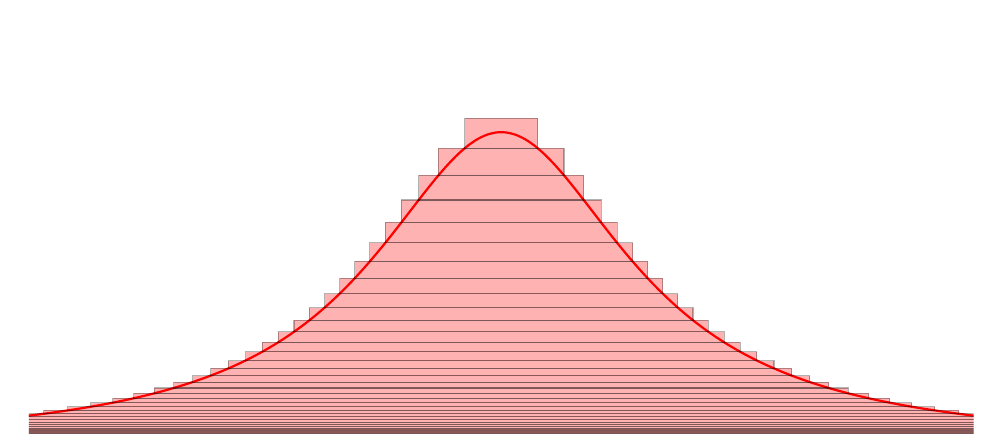
\begin{tikzpicture}
    \pgfmathdeclarefunction{f}{1}{\pgfmathparse{16/((#1)^2+4)}}
    \pgfmathdeclarefunction{g}{1}{\pgfmathparse{2*sqrt(4/(#1)-1)}}
    \draw (-6,0) -- (6,0);
    \draw[thick, smooth, red, domain=-6:6, samples=100] plot (\x,{f(\x)});
    \clip (-6,0) rectangle (6,4.8);
    \pgfmathsetmacro{\a}{1.1}
    \pgfmathtruncatemacro{\amin}{ceil(ln(0.01)/ln(\a))-1}
    \pgfmathtruncatemacro{\amax}{ceil(ln(4)/ln(\a))-1}
    \foreach \n in {\amin,...,\amax}
    {
        \draw[thin, fill=red, opacity=0.3] ({-g((\a)^(\n))},{(\a)^(\n)}) rectangle ({g((\a)^(\n))},{(\a)^(\n+1)});
    }
\end{tikzpicture}


Suppose 
Define $f_m(x)=f(x)^\ceil{\log_c(f(x))}$





\end{document}
